% ======================================================================
%  Supplementary Material / Appendix
%  VLM-Verified Counterfactual Hindsight for Sparse-Reward Manipulation
% ======================================================================

\section{Method Details and Environments}
\label{app:methods}

\paragraph{Cross-task VLM prompt template.}
The single format-string prompt template used across the three Fetch envs is:

\begin{quote}
\small
\texttt{You are an expert robotics analyst. The robot is attempting the
following task: \{task\_description\}. Examine the \{K\} keyframes of a
failed episode shown below. Identify the single keyframe index
$\in\{0,\dots,K\!-\!1\}$ at which the failure became inevitable, and a
1--2 sentence reasoning. Return strict JSON:
\{``failure\_frame\_index'': $i$, ``reasoning'': $s$\}.}
\end{quote}

\noindent
Per-env task-description substitutions:
\textbf{FetchPush:} ``the robot should push the red cube to the green target on the table'';
\textbf{FetchPickAndPlace:} ``the robot should pick up the red cube and place it at the floating green target'';
\textbf{FetchSlide:} ``the robot should strike the red puck so that it slides to the green target''.
The verified-CF mechanism uses an \textsc{action} variant of this
template that elicits a corrective 4-vector action sequence; full prompt
texts (four variants $\times$ task substitutions) and the
GoalDistanceLocalizer heuristic implementation are released at
\url{https://github.com/DJRGVC/RL_project_185}
(\texttt{src/vlm/prompts.py}; \texttt{src/vlm/verified\_counterfactual.py};
\texttt{src/vlm/oracle\_v3.py}).

\paragraph{Heuristic localizer (Oracle v3).}
The \texttt{GoalDistanceLocalizer} reads privileged sim state and selects
the failure timestep via three phases in precedence order:
\textbf{(a) ballistic}: latest contiguous run of $\ge\!3$ steps with
post-peak object velocity $>\!0.05$\,m/step (catches Slide free-flight);
\textbf{(b) contact-loss}: latest transition
$\text{in\_contact}_t\!\to\!\neg\text{in\_contact}_{t+1}$ with contact-run
length $\ge\!2$ and object-goal distance $>\!0.10$\,m
(catches Push/PnP drop-offs);
\textbf{(c) argmin}: closest-approach timestep as fallback. This serves
both as the supervised target for transfer evaluation and as the
privileged-state upper-envelope curve for Semantic PER.

\begin{figure}[t]
\centering
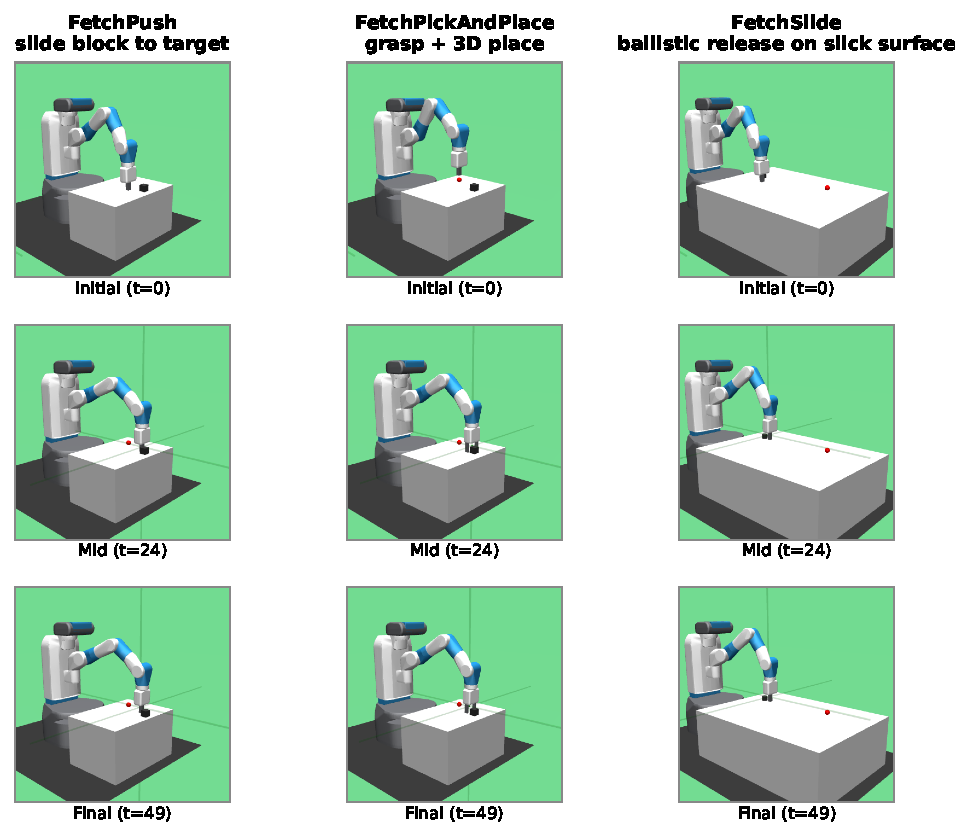
\includegraphics[width=\linewidth]{fig_envs.pdf}
\caption{The three Gymnasium-Robotics Fetch tasks used in our experiments
(columns: \texttt{FetchPush}, \texttt{FetchPickAndPlace},
\texttt{FetchSlide}), rendered at $t\!=\!0/24/49$ of a deterministic
scripted rollout (seed~42). Each task: 50-step horizon, 4-dim continuous
action (end-effector $\Delta xyz$ + gripper), sparse reward (binary,
success threshold 5\,cm to the green target).}
\label{fig:envs}
\end{figure}

\section{Bias-Bound Proof Sketch}
\label{app:bias-bound}

Let $\mathcal{L}_U(\theta)\!=\!\mathbb{E}_{i\sim U}[\ell(\delta_i)]$ be
the uniform-replay target loss. Standard PER with annealed correction
yields, in the $\beta_t\!\to\!1$ limit, an unbiased self-normalized IS
estimator of $\mathcal{L}_U$ \citep[Sec.~3.4]{schaul2016per}. Our Semantic
PER proposal $\mu_{\text{Sem}}\!\propto\!\mu_P\!\cdot\!w_{\text{sem}}$ is
a re-weighting of $\mu_P$ by a trajectory-conditional factor bounded by
$1\!\le\!w_{\text{sem}}\!\le\!w_{\max}$.
The strictly-correct IS weight is
$w_{\text{IS},\text{Sem}}(i)\!=\!(|\mathcal{D}_B|\mu_{\text{Sem}}(i))^{-\beta_t}$.
Our implementation under-corrects with $w_{\text{IS},P}$ (a V-trace-style
variance-reduction choice). The per-slot ratio is
$w_{\text{IS},P}/w_{\text{IS},\text{Sem}}\!=\!w_{\text{sem}}^{\beta_t}/Z^{\beta_t}$
where $Z$ is the $\mu_{\text{Sem}}$ normalizer. The window-kernel
structure of $w_{\text{sem}}$ confines the support of $w_{\text{sem}}\!>\!1$
to $2W\!+\!1$ slots out of $T$. Combining these gives
\begin{equation}
  \bigl|\widehat{\mathcal{L}}_{\text{under}} - \mathcal{L}_U\bigr|
  \;\le\;
  C\,\bigl(w_{\max}^{\,\beta_t} - 1\bigr)\,\frac{2W+1}{T}\,\|\ell\|_\infty,
  \label{eq:bias-bound}
\end{equation}
with $C$ a constant depending on $|\mathcal{D}_B|$ and the PER normalization.
At our defaults ($w_{\max}\!=\!10$, $W\!=\!5$, $T\!=\!50$,
$\beta_t\!\le\!1$) the bias multiplier is at most
$(10\!-\!1)\!\cdot\!11/50\!\approx\!1.98\,C\|\ell\|_\infty$, and
$\to\!0$ as $w_{\max}\!\to\!1$. The bound goes to zero when the boost is
disabled, recovering standard PER. The strictly-correct ablation (run
$w_{\text{IS},\text{Sem}}$) eliminates the residual bias entirely at the
cost of maintaining $Z$. \textbf{Two-regime degeneracy.} On the verifier
channel, miscalibration acts on
$m_\phi(\tau)\!=\!m_{\text{gen}}\!\cdot\!m_{\text{ver}}(\sigma)$
(VLM parse rate $\times$ verifier acceptance rate); the
$\varepsilon_{\text{cal}}\!=\!0$ guarantee holds vacuously when the
accepted set is empty (cold-start: $m_{\text{ver}}\!\to\!0$). Full
proof and the V-trace specialization derivation are at the GitHub URL above
(\texttt{paper/appendix\_theory.tex}).

\section{Hyperparameters and Compute}
\label{app:hparams}

\begin{table}[t]
\centering
\footnotesize
\caption{Headline hyperparameters. Full per-table breakdowns (SAC
architecture, HER strategy, PER schedule, Semantic-PER, Verified-CF, VLM
call) at the GitHub repo (\texttt{configs/}).}
\label{tab:hparams-headline}
\begin{tabular}{l l l}
\toprule
Parameter & Value & Notes \\
\midrule
\multicolumn{3}{l}{\textit{SAC} \citep{haarnoja2018sac}} \\
Hidden layers $\times$ width & $2 \times 256$, ReLU & Twin-Q critic; tanh-squashed Gaussian actor \\
LR (actor/critic/$\alpha$) & $3\!\times\!10^{-4}$ & Adam, default $(\beta_1,\beta_2,\varepsilon)$ \\
Discount $\gamma$ / Polyak $\tau$ & $0.98 / 0.005$ & Fetch-standard \\
Target entropy $\bar H$ & $-d_a\!=\!-4$ & Auto-tuned \\
Batch / updates per step & $256 / 1$ & 10k warm-up uniform-random \\
\midrule
\multicolumn{3}{l}{\textit{HER} \citep{andrychowicz2017her}} \\
Strategy / $k_{\text{HER}}$ & \texttt{future} / 4 & 4 hindsight transitions per real \\
\midrule
\multicolumn{3}{l}{\textit{PER} \citep{schaul2016per}} \\
$\alpha$ / $\beta_0\!\to\!\beta_{\text{end}}$ & $0.6 / 0.4\!\to\!1.0$ & Linear over 500k steps; $\varepsilon\!=\!10^{-6}$ \\
\midrule
\multicolumn{3}{l}{\textit{Semantic PER}} \\
Window half-width $W$ & 5 timesteps & $11$-slot box around $t_{\text{fail}}$ \\
Boost cap $w_{\max}$ & 10 & Multiplicative factor on PER priority \\
Keyframes $K$ / VLM provider & 5 / GPT-4o (production) & \texttt{gpt-4o-2024-08-06} \\
\midrule
\multicolumn{3}{l}{\textit{Verified-CF}} \\
Verifier rollout horizon $N$ & 50 steps & One Fetch episode \\
Success threshold $\eta$ / teleport reject $\rho$ & $0.05 / 0.05$\,m & Env's native threshold \\
CF prompt variant & \textsc{action} & Structurally teleport-immune \\
\midrule
\multicolumn{3}{l}{\textit{Training}} \\
Total env steps & 500k (paper-grade) & 250k--1M for selected ablations \\
Random seeds & 42, 123, 999 & 3 per (method, env) cell \\
Replay capacity & $10^6$ slots & Ring buffer with sum-tree priorities \\
\bottomrule
\end{tabular}
\end{table}

\paragraph{Compute.}
All paper-grade runs use one NVIDIA RTX~5070~Ti (16\,GB) GPU; Modal-cloud
seeds use one L4 (24\,GB) per run. Per-run wall-clock at 500k steps:
$\approx\!6$h SAC+HER, $\approx\!9$h SAC+HER+VLM-CF (extra time is
VLM-API latency, not compute). Total project compute:
$\sim$220 GPU-hours across local + Modal, plus
$\sim\!\$80$ VLM-API spend. Snapshot round-trip latency for the
verifier is 17.6\,ms per call (a $0.4\%$ overhead at $\sim\!1700$ failed
episodes / 100k steps). Reproduction commands, W\&B run-IDs, and
per-seed eval traces are at
\url{https://github.com/DJRGVC/RL_project_185} (commit \texttt{0fa36fc}).

\section{Additional Experimental Detail}
\label{app:results}

\paragraph{Real-data validation (extended).}
The $n\!=\!10$ real-failure dataset consists of failed eval episodes from
partially-trained SAC+HER checkpoints (\texttt{FetchPickAndPlace} at
50k steps, \texttt{FetchPush} at 30k steps, both at $\sim\!5\%$ eval
success). Real failures are near-misses with final-distance
$\in\!\![0.06,0.34]$\,m on Push and median $0.27$\,m on PickAndPlace
(contact-task failures, not the block-flies-off-table synthetic mode).
Three findings transfer to production:
\textbf{(i) Teleport-collapse persists and is task-conditioned.} On Push
(planar target), Opus and Sonnet teleport on \textsc{achieved\_goal} at
$100\%$ and $75\%$; on PickAndPlace (mid-air target), Opus teleports at
$75\%$ but Sonnet drops to $0\%$, proposing a mid-air waypoint
$\sim\!8$\,cm above the floating goal. Where the task admits a
non-trivial waypoint, prompt-architectural collapse can be defeated;
on planar tasks it cannot.
\textbf{(ii) The 5\,cm reject-teleport gate is structurally necessary.}
Aggregated across both VLMs and both position-emitting variants on $20$
generations, the gate fires on $12$ ($60\%$); the cross-vendor floor on
Push is $75\%$. The action-emitting verifier sidesteps this entirely.
\textbf{(iii) Plausibility shifts only $\pm 0.07$ synthetic-to-real, but
the \textsc{action} sign-flip rate worsens} (Opus $0.50\!\to\!0.55$,
Sonnet $0.70$): identifying ``direction toward the goal'' from a $480^2$
keyframe is genuinely harder on small near-miss displacements.

\paragraph{Statistical methodology.}
Each (method, env) cell uses $n\!=\!3$ seeds (42, 123, 999); reported
metrics are mean~$\pm$~SE computed across seeds using the
$t$-distribution with $n\!-\!1\!=\!2$ d.f. Statistical comparison
statements use non-overlapping SE intervals as the threshold (a
conservative two-sample criterion at this sample size).
The load-bearing $0/6$ vs.\ $4/4$ contrast in Table~\ref{tab:prompt-variants}
is decided by Euclidean predicate (judge-independent) and Fisher's
exact test rejects equal-proportions at $p\!<\!0.005$.

\paragraph{Cross-task transfer (per-episode notes).}
A 12-episode pilot ($4$ per env). The VLM's reasoning strings
identify task-specific modes correctly in every case---Push:
\emph{``gripper passes over block without making contact''};
PickAndPlace: \emph{``gripper at block location but fails to close''};
Slide: \emph{``strike direction off-axis''}. The $2/4$ PickAndPlace
keyframe-agreement reflects heuristic under-localization (closed-loop
grip timing is the hardest mode for geometry-only oracles
\citep{sayar2023cebp}) rather than VLM error: the VLM assigns the failure
frame one step earlier at the decisive grip sequence, a different but
arguably more physically-correct localization.

\section{Broader Impacts and Reproducibility}
\label{app:impact}

\paragraph{Broader impact.}
This work is methodological and simulation-only; we make no claims about
real-robot performance, sim-to-real transfer, or any specific deployment
scenario.
\emph{Positive aspects.}
(i)~Reduced sample requirements lower the energy footprint of
robot-learning research: fewer environment steps means fewer GPU-hours.
(ii)~The IS-posterior framing provides a principled lens for the
emerging class of VLM-in-replay methods.
(iii)~The verified-CF acceptance gate is a general-purpose
``language prior $+$ physics test'' pattern that may transfer to
program-synthesis verification or constraint-satisfaction guidance.
\emph{Negative aspects and mitigations.}
(i)~Foundation-model API use carries non-trivial energy and dollar cost
per training run; we mitigate by reporting per-run API spend (this
appendix) and providing the heuristic Oracle fallback that requires no
API calls.
(ii)~The VLM may hallucinate physically implausible corrective actions;
the simulator-verification gate is our primary mitigation---a
hallucinated action that does not satisfy the env's sparse reward is
rejected before entering the buffer.
(iii)~No robot-deployment safety risks are introduced beyond standard
simulation-trained policy deployment caveats.

\paragraph{Reproducibility.}
All training scripts, configurations, analysis notebooks, the full
appendix material (algorithm pseudocode for Semantic PER and
Verified-CF; full prompt-variant texts; V-trace/Retrace specialization;
two-regime $q_\phi$ degeneracy proof; reproducibility checklist;
extended limitations) are released at
\url{https://github.com/DJRGVC/RL_project_185}
(commit \texttt{0fa36fc}). The verified-CF prototype lives at
\texttt{src/vlm/verified\_counterfactual.py}; the Semantic-PER buffer at
\texttt{src/buffers/semantic\_per.py}; reproduction commands at
\texttt{REPRODUCE.md}; W\&B run IDs (
\texttt{path\_c\_overnight}) and per-seed eval traces are linked from
the README. The Sharony VLM-RB \citep{sharony2026vlmrb} reproduction
(faithful to their priority formula, $\lambda$-schedule, and clip length,
substituting Claude Sonnet~4.5 for the API-inaccessible PerceptionLM-1B)
is pre-staged at \texttt{src/buffers/vlm\_rb\_buffer.py} for
camera-ready head-to-head evaluation.
